\chapter{基础数据}\label{基础数据}
%\addcontentsline{toc}{chapter}{地表输入数据}


\section{高程数据}
高程数据来自MERIT DEM数据集 \citep{yamazaki2017high}。该数据集是通过从已有的遥感DEM (SRTM3 v2.1和AW3D-30m v1) 中去除多种误差 (绝对偏差、条纹噪声、散斑噪声和树高偏差) 而开发的,它的分辨率为3秒 (赤道处约90米) ,覆盖了90N-60S之间的陆地区域。

\section{地表覆盖数据}\label{地表覆盖数据}
\subsection{USGS地表覆盖数据}\label{USGS地表覆盖数据}
USGS地表覆盖数据来自美国地质调查局(USGS),数据全称为Global Land Cover Characterization (GLCC) database Version 2.0 
(\url{https://www.usgs.gov/centers/eros/science/usgs-eros-archive-land-cover-products-global-land-cover-characterization-glcc})。
数据为全球 \ang{;;30} (约1公里) 分辨率,经纬度网格,单时次数据,划分类型如表~\ref{tab:USGS覆盖类型} 所示。
% Please add the following required packages to your document preamble:
% \usepackage{booktabs}
\begin{table}[]
\centering
\caption{USGS覆盖类型}
\label{tab:USGS覆盖类型}
\begin{tabular}{@{}ll@{}}
\toprule
编号 & USGS覆盖类型     \\ \midrule
1  & 城市           \\
2  & 干旱农田与牧场      \\
3  & 灌溉农田与牧场      \\
4  & 干旱/灌溉混合农田与牧场 \\
5  & 农田草地过渡带      \\
6  & 农田林地过渡带      \\
7  & 草地           \\
8  & 灌木地          \\
9  & 草地灌木地混合带     \\
10 & 稀疏草原         \\
11 & 落叶阔叶林        \\
12 & 落叶针叶林        \\
13 & 常绿阔叶林        \\
14 & 常绿针叶林        \\
15 & 混合森林         \\
16 & 内陆水体         \\
17 & 草本湿地         \\
18 & 森林湿地         \\
19 & 贫瘠稀疏植被       \\
20 & 草本苔原         \\
21 & 森林苔原         \\
22 & 混合苔原         \\
23 & 裸土苔原         \\
24 & 雪盖或冰川        \\ \bottomrule
\end{tabular}
\end{table}


由于USGS地表覆盖数据为单时次且年代稍远(主要数据源自AVHRR 1992-1993年间),因此辅以其他特定类型地表覆盖数据对USGS地表覆盖进行更新。
包括全球1公里水体和湿地数据(Global Lakes and Wetlands Database: Lakes and Wetlands Grid (Level 3))~\citep{lehner2004development}、
全球1公里冰川数据~\citep{RGIConsortium2017}、全球1公里城市覆盖数据 (MODIS)~\citep{schneider2009new} 和全球1公里高程数据(USGS)。
替换方式是将以上辅助数据中水体、冰川和城市网格直接对USGS地表数据进行替换。USGS高程数据用于判断海洋,即将高程低于0米的地方设置为海洋格点。
如采用USGS地表覆盖类型进行模拟 (LCT方案),其不同类型相关参数请参考附录~\ref{USGS地表覆盖类型相关参数}。

\subsection{IGBP地表覆盖数据}\label{IGBP地表覆盖数据}
IGBP地表覆盖数据来自美国宇航局(NASA)Moderate Resolution Imaging Spectroradiometer 
(MODIS)MCD12Q1 Version 6(The Terra and Aqua combined MODIS Land Cover Type data product)
的数据(\url{https://lpdaac.usgs.gov/products/mcd12q1v006/}),该数据(LC\_Type1)是Terra和Aqua两种卫星数据结合产生 
 \citep{Friedl2019}。数据为全球 \ang{;;15}(约500 m)分辨率,经纬度网格(对原始数据做了投影转换),每年一幅数据,时间范围从2001至今,分类如表 \ref{tab:IGBP覆盖类型} 所示。

\begin{table}[]
\centering
\caption{IGBP覆盖类型}
\label{tab:IGBP覆盖类型}
\begin{tabular}{@{}ll@{}}
\toprule
编号 & IGBP覆盖类型     \\ \midrule
1  & 常绿针叶林           \\
2  & 常绿阔叶林      \\
3  & 落叶针叶林     \\
4  & 落叶阔叶林 \\
5  & 混合林     \\
6  & 郁闭灌丛      \\
7  & 稀疏灌丛           \\
8  & 稀疏大草原(木本为主)         \\
9  & 稀疏大草原     \\
10 & 草地         \\
11 & 永久性湿地        \\
12 & 耕地        \\
13 & 城市        \\
14 & 耕地和自然植被混合带        \\
15 & 积雪和冰川        \\
16 & 裸土或稀疏植被覆盖       \\ 
17 & 水体           \\ \bottomrule
\end{tabular}
\end{table}


\section{土壤数据}\label{土壤数据}
\subsection{土壤基础属性}\label{土壤基础属性}
土壤基础属性数据采用Global Soil Dataset for Earth System Modeling(GSDE,\url{http://globalchange.bnu.edu.cn/research/soilw})~\citep{shangguan2014global}
和SoilGrids(\url{https://www.soilgrids.org/})\citep{poggio2021soilgrids} 两套数据。GSDE采用土壤连接法融合了世界土壤图和多个区域级或国家级的土壤数据库,基于土壤剖面和土壤类型图生成。其空间分辨率为1公里。其垂直层次为8层 (0--0.045, 0.045--0.091, 0.091--0.166, 0.166--0.289, 0.289--0.493, 0.493--0.829, 0.829--1.383, 1.383--2.296 m),这一分层方案与CoLM一致(第一层对应CoLM第一和第二层)。SoilGrids基于土壤剖面和数百个环境协变量图层采用基于机器学习的数字土壤制图方法生成,空间分辨率为250 m。其垂直层次为6层(0--0.05,0.05--0.15,0.15--0.3,0.3--0.6,0.6--1,1--2 m)。对两个数据按CoLM的土壤分层方案采用深度加权方法进行了标准化处理。其中第十层无数据,用第九层填补。

\subsection{基岩深度}\label{基岩深度}

基岩深度数据来自Global Depth to Bedrock Dataset for Earth System Modeling (GDBDESM,\url{http://globalchange.bnu.edu.cn/research/dtb.jsp}, \citet{shangguan2017mapping})。该数据集基于土壤剖面、地质钻孔和环境协变量图层采用机器学习的数字土壤制图方法生成,空间分辨率为1公里。


\section{植被结构及属性数据}\label{植被结构及属性数据}
\subsection{叶面积指数数据}\label{叶面积指数数据}
叶面积指数数据来自重处理的MODIS LAI数据~\citep{yuan2011reprocessing}。目前模式提供MODIS第5版和第6.1版数据。其中MODIS第5版数据 (MOD15A2) 为全球 \ang{;;30} (1公里) 分辨率,经纬度网格,时间覆盖2000--2016年,时间分辨率为每8天。MODIS第6.1版数据 (MCD15A2H),空间分辨率为全球 \ang{;;15} (约500米),经纬度网格,时间覆盖从2000年至今,时间分辨率每8天或每月。


\subsection{树高数据}\label{树高数据}
树高数据来自2005年Geoscience Laser Altimeter System (GLAS) aboard ICESat 
(Ice, Cloud, and land Elevation Satellite)卫星数据~\citep{simard2011mapping},
全球 \ang{;;30} (1公里) 分辨率,经纬度网格,单时次数据。

\subsection{PFT/PC数据及其依赖数据}\label{PFTPC数据及其依赖数据}
模式如采用PFT或PC植被次网格方式运行,则不能像LCT方案一样直接进行地表覆盖类型聚合(图~\ref{fig:次网格聚合方案} LCT方案所示),
需要对每一个细网格地表覆盖类型进行拆解,得到其网格内PFT的组成种类和各自面积占比。
PFT方案则根据细网格计算得到的PFT种类及占比来聚合到模式网格(图~\ref{fig:次网格聚合方案} PFT方案)。
PC聚合方案同LCT,但是PC跟PFT方案一样,对每种LCT内的PFT进行表征 (包括类型和组成比例,图~\ref{fig:次网格聚合方案} PC方案)。
PFT和PC方案采用同样的植被功能型分类,如表~\ref{tab:PFT分类} 所示:
% Please add the following required packages to your document preamble:
% \usepackage{booktabs}
\begin{table}[htbp]
\centering
\caption{植被功能型-PFT分类}
\label{tab:PFT分类}
\begin{tabular}{ll}
\toprule
\multicolumn{1}{l}{编号} & \multicolumn{1}{l}{植被功能型} \\ \midrule
0                      & 裸土                        \\
1                      & 温带常绿针叶树                   \\
2                      & 北方常绿针叶树                   \\
3                      & 北方落叶针叶树                   \\
4                      & 热带常绿阔叶树                   \\
5                      & 温带常绿阔叶树                   \\
6                      & 热带落叶阔叶树                   \\
7                      & 温带落叶阔叶树                   \\
8                      & 北方落叶阔叶树                   \\
9                      & 常绿阔叶灌木                    \\
10                     & 温带落叶阔叶灌木                  \\
11                     & 北方落叶阔叶灌木                  \\
12                     & 极地C3草                     \\
13                     & C3草                       \\
14                     & C4草                       \\
15                     & C3作物                      \\ \bottomrule
\end{tabular}
\end{table}

{
\begin{figure}[htbp]
\centering
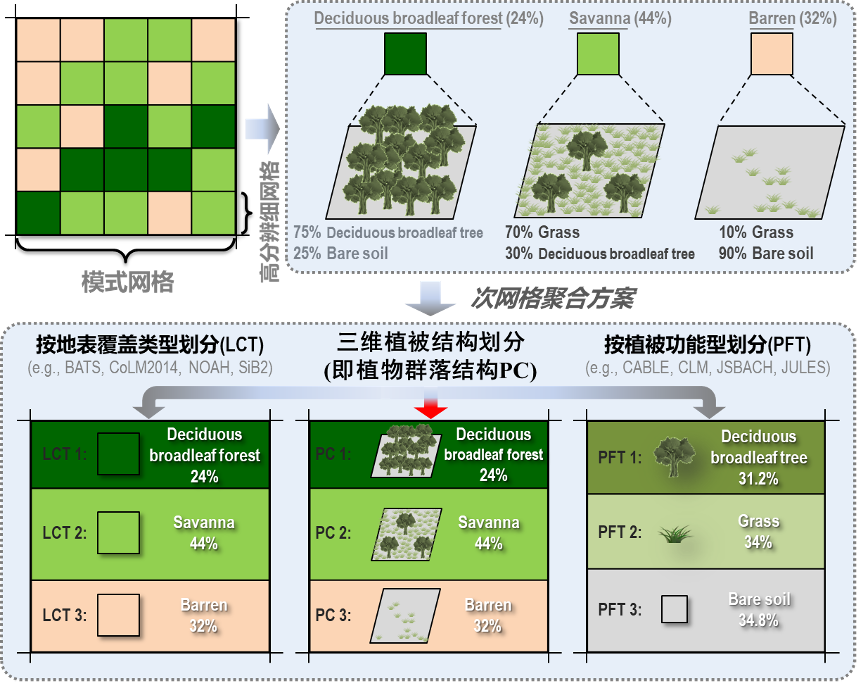
\includegraphics{Figures/基础数据/次网格聚合方案.png}
\caption{CoLM三种植被次网格聚合方案 (LCT、PC和PFT) 示意图。}
\label{fig:次网格聚合方案}
\end{figure}
}


由于PFT和PC方案都需要对细网格地表覆盖数据进行PFT分解,而地表覆盖原数据并不包含此信息,
需要借助辅助数据进行计算,其数据来源如表~\ref{tab:网格划分辅助数据} 所列。

% Please add the following required packages to your document preamble:
% \usepackage{booktabs}
% \usepackage[table,xcdraw]{xcolor}
% If you use beamer only pass "xcolor=table" option, i.e. \documentclass[xcolor=table]{beamer}
\begin{landscape}
\begin{table}[htbp]
%\begin{sidewaystable}[]
\centering
\caption{用于PFT和PC次网格划分辅助数据}
\label{tab:网格划分辅助数据}

\begin{tabular}[h]{p{3cm}p{6cm}p{2cm}p{2cm}p{5cm}}
\toprule
数据名称      & 描述        & 分辨率   & 坐标投影     & 参考文献           \\ \midrule
MODIS Land Cover Type & The Terra and Aqua combined MODIS Land Cover Type (LC\_Type1) data product, Version 6 (MCD12Q1) & 500 m & Sinusoidal        & \citet{Friedl2019}                \\\midrule
ESA LC-CCI land cover type         & ESA CCI land cover type products                                                                & 300 m & Latitude-Longitude & \url{http://maps.elie.ucl.ac.be} \\\midrule
MODIS VCF      & MODIS Vegetation Continuous Fields product, Version 6 (MOD44B)                                           & 250 m    & Sinusoidal         & \citet{DiMiceli2015}                        \\\midrule
AVHRR VCF& AVHRR Tree Cover (evergreen, deciduous and broadleaf, needleleaf) Continuous Fields                      & 1 km  & Latitude-Longitude & \citet{defries2000new}                         \\\midrule
Köppen-Geiger climate classification        & Present Köppen-Geiger climate classification maps at 1-km resolution                            & 1 km  & Latitude-Longitude & \citet{beck2018}     \\\midrule
Reprocessed MODIS LAI                 & Reprocessed MODIS leaf area index produces, Version 6                                           & 500 m & Sinusoidal         & \citet{yuan2011reprocessing}     \\\midrule
WorldClim Version2                    & Worldclim 2: New 1-km spatial resolution climate surfaces for global land areas                          & 1 km  & Latitude-Longitude & \citet{fick2017worldclim}   \\\midrule
Canopy height                         & Global 1 km forest canopy height map                                                            & 1 km  & Latitude-Longitude & \citet{simard2011mapping}             \\ \bottomrule
\end{tabular}
%\end{sidewaystable}
\end{table}
\end{landscape}
如采用PFT/PC方案进行植被次网格模拟,其不同类型相关参数请参考附录~\ref{植被功能型PFT相关参数} 和附录~\ref{植物群落PC次网格PFT相关参数}。


\section{水文数据}\label{水文数据}
\subsection{水文学基础数据}
\subsection{河网}
CaMa-Flood 模拟所需的相关次网格地形参数是由 90m 超高精细分辨率的全球流动方向地图 (MERIT-Hydro)\citep{yamazaki2019merit},
水文调整高程 DEM~\citep{yamazaki2017high,yamazaki2012analysis},以及河宽数据~\citep{yamazaki2014development}; 
使用 \citet{yamazaki2009deriving} 开发的升尺度模式 Flexible Location of Waterways (FLOW) 计算得出。
相关数据以纯``二进制''格式 ($nx\times ny$)存储于 \texttt{map/} 目录下。默认的数据存储顺序是从180 \textdegree W到180 \textdegree E,
从 90 \textdegree N 到 90 \textdegree S;数据的字节顺序是'little endian'。
具体而言,除了需要陆面模式计算得出的产流量 (runoff) 之外,CaMa-Flood还需要包括流域面积 ($A_s$),河道长度 ($L$),河道宽度 ($W$) 及深度 ($B$),
漫滩 (洪水淹没) 面积,以及用于计算平均漫滩水深的漫滩高程剖面等相关的次网格地形数据。除了河流的宽度和深度以外,
所有的地形相关参数均可由 MERIT-hydro 水文地形数据中获取。以下以全球~0.25\textdegree ~的河网为例进行详细介绍。

{
\begin{figure}[]
\centering
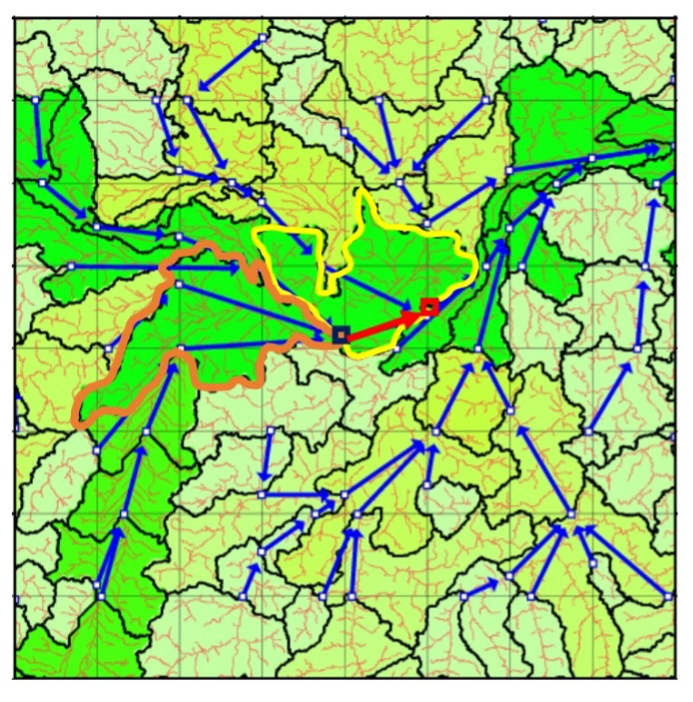
\includegraphics{Figures/陆地表面的水分循环/流域单元分布图.png}
\caption{流域单元分布图。每个流域单元的出口用白色四边形标记。蓝色线条连接不同流域单元,箭头指向下游流域单元。
橙色和黄色边界代表了不同的流域单元。图片摘自\citet{yamazaki2013improving}。 }
\label{fig:流域单元分布图}
\end{figure}
}


在目录\texttt{glb\_15min}下包含了全球 0.25\textdegree 分辨率的网格-矢量-混合 (grid-vector-hybrid) 河网图,
该河网地图是由 90m MERIT Hydro 数据使用 FLOW 模式升尺度而来 (图~\ref{fig:流域单元分布图});
具体文件内容如表~\ref{tab:河网图及地形参数文件列表} 和表~\ref{tab:河网图及地形参数文件列表2} 所示。
河网地图的维度信息,包括东西方向网格数目$nx$,南北方向网格数目$ny$,泛滥平原层数 ($nfpl$),
网格大小 ($gsize$)和区域边界 (西、东、南、北),记录在 \texttt{params.txt} 之中。\texttt{nextxy.bin} 文件包含了2个参数 ($nextx$和$nexty$),
分别记录了每个网格的下游单元的相对位置,
其中与海洋接口的河口标记为 -9,内陆河流终点标记为 -10,海洋 (未定义) 标记为 -9999。

% Please add the following required packages to your document preamble:
% \usepackage{booktabs}
\begin{table}[]
\centering
\caption{河网图及地形参数文件列表}
\label{tab:河网图及地形参数文件列表}
    \begin{tabular}[h]{p{3.5cm}p{1.5cm}p{1.5cm}p{5cm}p{1cm}p{1cm}}  %{@{}cccccc@{}}
    \toprule
    File              & Variable & Symbol                        & Description                                  & Unit    & Format  \\ \midrule
    \texttt{params.txt}        & -        & -                             & Map parameters                     & -         & text    \\
    \texttt{nextxy.bin}        & \texttt{nextx}    & $jx$                         & Downstream X (rec=1)         & -         & integer \\
                                       & \texttt{nexty}    & $jy$                         & Downstream Y (rec=2)            & -        & integer \\
    \texttt{downxy.bin}      & \texttt{downx}   & $dx$                        & Relative DownstreamX (rec=1)   & -   & integer \\
                                       & \texttt{downy}   & $dy$                      & Relative Downstream Y (rec=2)   & -    & integer \\
    \texttt{ctmare.bin}       & \texttt{ctmare}   & $Ac$                     & Unit-catchment Area                     & $\rm m^2$   & real    \\
    \texttt{elevtn.bin}        & \texttt{elevtn}    & $Z$                        & Base Elevation                         & m       & real    \\
    \texttt{rivlen.bin}         & \texttt{rivlen}    & $L$                         & Channel Length                        & m       & real    \\
    \texttt{rivhgt.bin}         & \texttt{rivhgt}   & $B$                         & Channel Depth                          & m       & real    \\
    \texttt{rivwth.bin}        & \texttt{rivwth}   & $W$                        & Channel Width                           & m       & real    \\
    \texttt{rivwth\_gwdlr.bin} & \texttt{rivwth}   & $W$                    & Combined Width (recommended)    & m       & real    \\
    \texttt{nxtdst.bin}        & \texttt{nxtdst}   & $X$                             & Downstream Distance                          & m       & real    \\
    \texttt{fldhgt.bin}        & \texttt{fldhgt}   & $D_f$                            & Floodplain Elevation profile (rec=1$\sim$10) & m       & real    \\
    \texttt{rivman.bin}        & \texttt{rivman}   & -                             & Manning’s Roughness                          & -       & real    \\
    \texttt{bifori.txt}        & -        & -                             & Bifurcation Channel Original Data            & -       & text    \\
    \texttt{bifprm.txt}        & -        & -                             & Bifurcation channel parameters               & -       & text    \\ \bottomrule
    \end{tabular}
\end{table}


    % Please add the following required packages to your document preamble:
% \usepackage{booktabs}
\begin{table}[]
\centering
\caption{河网图及地形参数文件列表续}
\label{tab:河网图及地形参数文件列表2}
    \begin{tabular}[h]{p{3.5cm}p{1.5cm}p{1.5cm}p{5cm}p{1cm}p{1cm}} %{@{}cccccc@{}}
    \toprule
    File             & Variable & Symbol                             & Description                                          & Unit     & Format  \\ \midrule
    \texttt{grdare.bin}       & \texttt{grdare}   & -                                  & Rectangular grid area (optional)                     & \unit{m^2}       & real    \\
    \texttt{nxtdst\_grid.bin} &          &                                    &                                                      &          &         \\
    \texttt{rivlen\_grid.bin} & \texttt{nxtdst}   & $X$                                  & Downstream Distance (grid center)                    & m        & real    \\
                                        & \texttt{rivlen}    & $L$                            & Channel Length (grid center)       &    m                             & real        \\
    \texttt{inpmat.bin}       & \texttt{inpx}     & -                                  & Corresponding input grid X (rec=1) & -        & integer \\
                                       & \texttt{inpy}     & -                               & Corresponding input grid Y (rec=2)    & -        & integer  \\
    \texttt{ctmare.bin}       & \texttt{inpa}     & $A_{ij}$                            & Area of input grid XY (rec=3)              & \unit{m^2}     & real    \\
    \texttt{diminfo.txt}      & -        & -                                  & Dimension infomation                         & text     &         \\
    \texttt{lsmask.bin}       & -        & -                                  & Land ID of corresponding hi resolution area Basin ID & -        & integer \\
    \texttt{basin.bin}        & -        & -                                  & Basin ID                                             & -        & integer \\
    \texttt{bsncol.bin}       & -        & -                                  & Basin Color Pattern for Visualization                & -        & integer \\
    \texttt{lonlat.bin}       & \texttt{lon}      & -                                  & Longitude, catchment outlet (rec=1)     & \textdegree      & real    \\
                                     & \texttt{lat}       & -                                 & Latitude, catchment outlet (rec=2)        & \textdegree       & real    \\
    \texttt{uparea.bin}       & \texttt{uparea}   & -                           & Upstream Drainage Area                       & \unit{m^2}        & real    \\ \bottomrule
    \end{tabular}
\end{table}


假设任意网格的洪水事件是从高程低的区域到高程高的区域发生淹没,
任意流域单元(图~\ref{fig:基于流域单元的漫滩高程剖面函数}) 的漫滩面积可以由漫滩水深$D_f$ (m) 
以及累积分布函数 (CDF) 的经验函数生成 (图~\ref{tab:河网图及地形参数文件列表2})。
每个网格的CDF函数的第10百分位数的10个值 (图~\ref{tab:河网图及地形参数文件列表2},红色圆点)分别存储在 \texttt{fldhgt.bin} 的十个参数之中
 (见表~\ref{tab:河网图及地形参数文件列表} 和表~\ref{tab:河网图及地形参数文件列表2}),文件格式与上述的 \texttt{nextxy.bin} 相同。
例如,\texttt{fldhgt.bin} 的第三个参数表示流域单元 30\% 的面积被淹没时的该流域单元的平均洪水深度 (m)。

{
\begin{figure}[htbp]
\centering
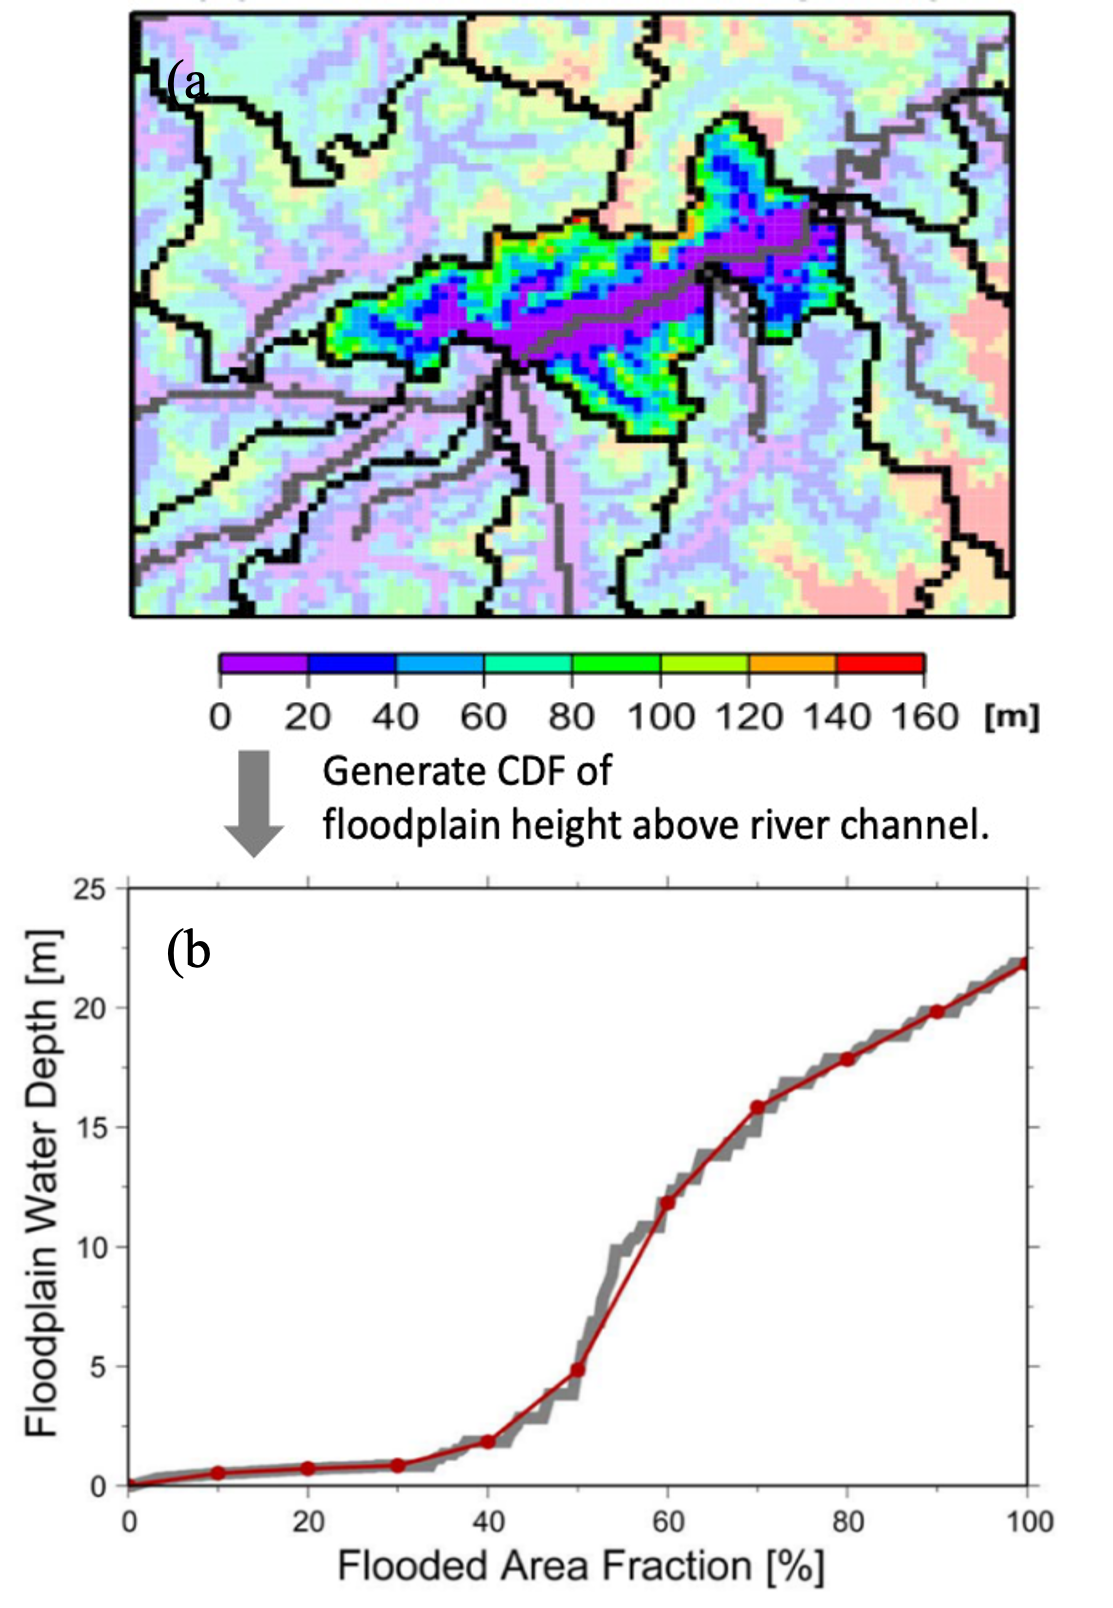
\includegraphics{Figures/陆地表面的水分循环/基于流域单元的漫滩高程剖面函数.png}
\caption{基于流域单元的漫滩高程剖面函数。图片摘自\citet{yamazaki2013improving}。  }
\label{fig:基于流域单元的漫滩高程剖面函数}
\end{figure}
}


河道断面参数(河道长度$W$ (m)和河道深度 $B$ (m))是水动力模拟的主要参数之一。在CaMa-Flood中的该参数是流域产流量的气候态的经验函数,由以下公式推导得出:
\begin{equation}
W=\max \left(W_{min}, c_{w} * Q_{ave}{}^{p_{w}}+W_{0}\right)
\end{equation}
\begin{equation}
B=\max \left(B_{min}, c_{H} * Q_{ave}{}^{p_{H}}+B_{0}\right)
\end{equation}
其中$Q_{ave}$是由陆面模式计算得出的产流量 (total runoff) (\unit{m^3.s^{-1}})。
河道宽度计算所使用的经验系数 $c_w$,$p_w$,$W_0$,$W_{min}$ 分别设置为 2.5,0.6,0.0 以及5.0;
河道深度计算所使用的经验系数 $c_H$,$p_H$,$B_0$ 和 $B_{min}$ 分别设置为 0.1,0.5,0.0 以及1.0。
值得注意的是这些经验系数存在着极大的不确定性,在使用之时需要对其进行对应的率定和调参。
除此之外,基于卫星观测的河道宽度数据 (\texttt{width.bin},如图~\ref{fig:基于卫星数据生成的河道宽度示意图}) 也可由MERIT-hydro水文地形数据中获取。
CaMa-Flood推荐使用通过 \texttt{set\_gwdlr.F90} 子程序生成组合宽度参数 (经验公式和卫星数据的组合) 数据。
相关地图的制备详见 \citet{yamazaki2014regional, yamazaki2014development}。

{
\begin{figure}[htbp]
\centering
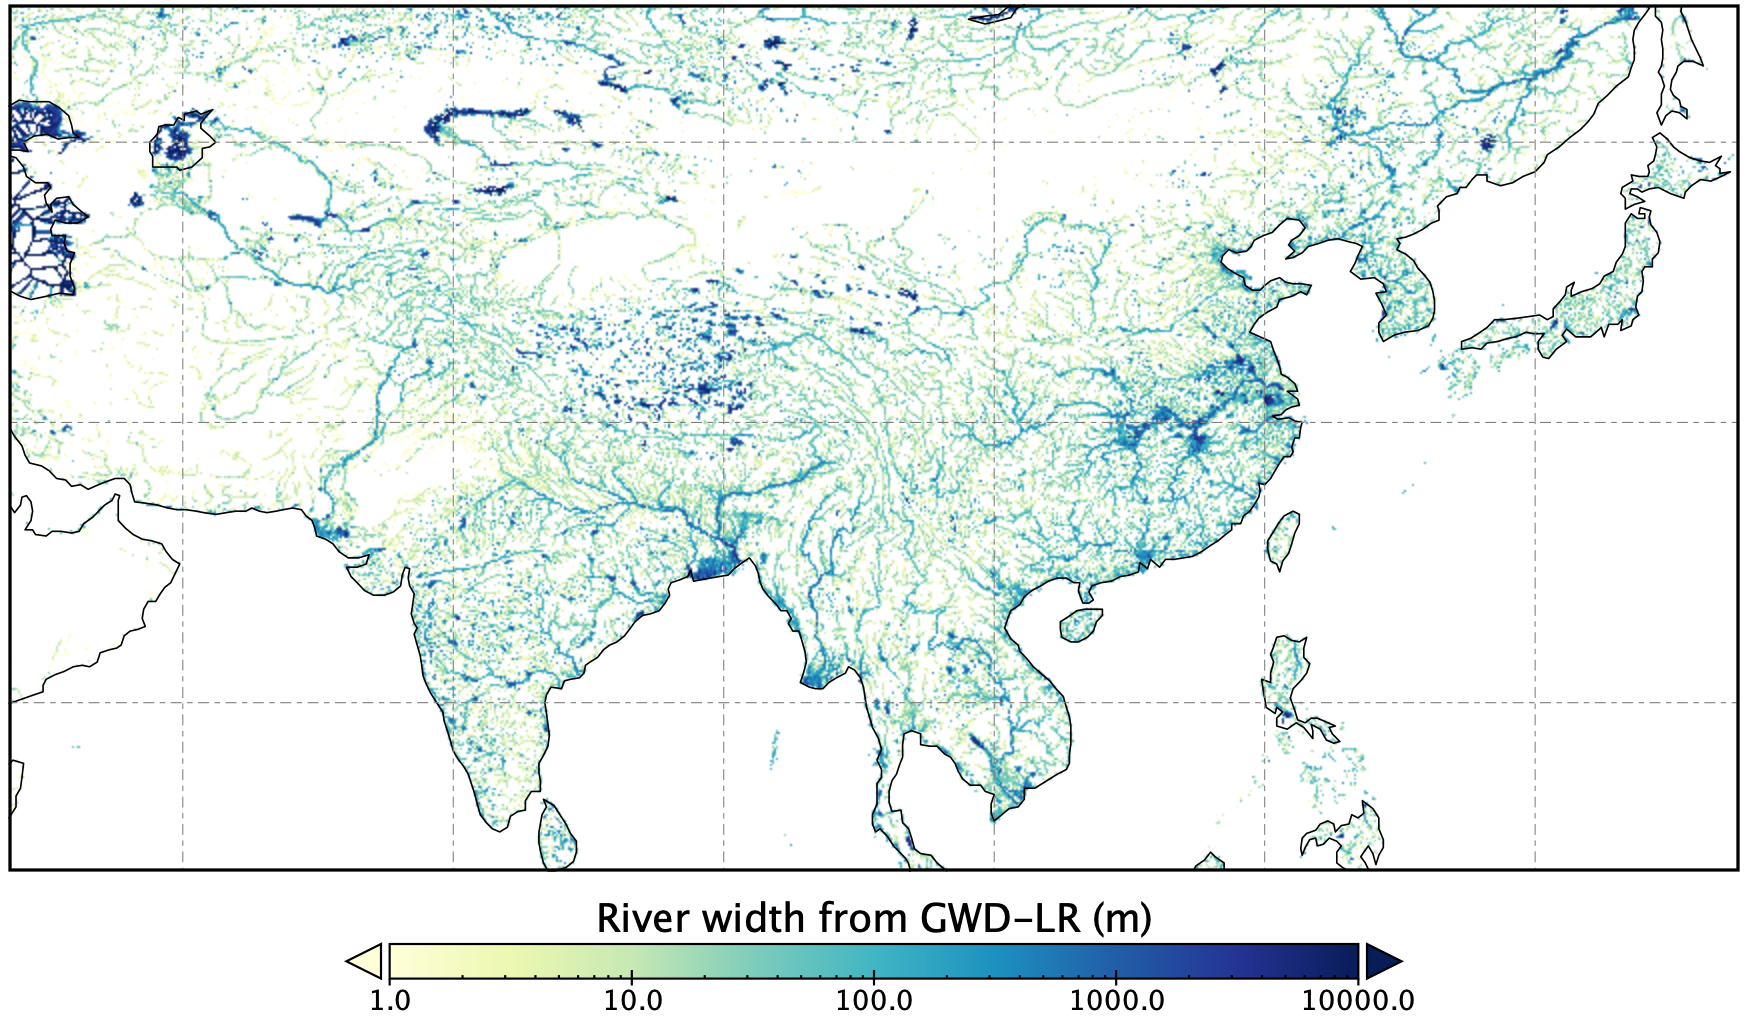
\includegraphics{Figures/陆地表面的水分循环/基于卫星数据生成的河道宽度示意图.png}
\caption{基于卫星数据生成的河道宽度示意图。图片摘自\citet{yamazaki2011physically}。}
\label{fig:基于卫星数据生成的河道宽度示意图}
\end{figure}
}

如图~\ref{fig:流域单元分布图} 所示,由于 CaMa-Flood 是基于流域单元进行计算的,而陆面模式是基于规则的经纬度网格,
流域单元在当前陆面模式分辨率 (经纬度网格) 投影下呈现不规则的形状。
因此在流域边缘有可能出现一个网格分属于不同流域,以及多个经纬度网格单元同属于一个流域单元的情况。
这就需要强制插值分割这些陆面模式经纬度网格生成的产流量到不同的流域。
指定流域单元$i$从陆面模式网格获得的水量由如下公式进行计算:
\begin{equation}
F_{i}=\sum_{N} A_{i, j} R_{j}
\end{equation}
其中$F_i$为进入流域单元$i$在单位时间 [\unit{m^3.s^{-1}}]的输入水量,$A_{i, j}$ 是陆面模式的经纬度网格单元$j$在属于指定流域单元的面积大小,
 $N$是指属于指定流域单元陆面模式的经纬度网格的数量。该映射信息被存储在 \texttt{test\_***.bin} (\texttt{***} 是网格分辨率
 ,例如 \texttt{test\_1deg.bin})。同时,还需准备一个文本文件 (比如说 \texttt{diminfo\_test-1deg.txt}) 用来指定模拟的维度
  (比如说区域,分辨率,流域单元数量,输入经纬度网格数量,输入的映射文件名 \texttt{test\_***.bin})。

在 \texttt{map} 目录中,CaMa-Flood 还准备了一些用于生成映射矩阵和漫滩高程剖面曲线所需的高分辨率数据 (如 \texttt{3sec},\texttt{1min},\texttt{15min},
\texttt{3min} 等目录之下)。
高分辨率数据被划分为\texttt{\$(TILE).\$(VAR).bin},每个TILE的区域记录在 \texttt{location.txt} 文件之中;
具体提供的参数 \texttt{\$(VAR)} 如表~\ref{tab:河网图及地形参数文件列表2} 所示。其中 \texttt{\$(TILE).flwdir.bin} 和
\texttt{\$(TILE).downxy.bin} 分别以基于 D8 格式和 downstreamXY 格式描述了河流流向;\texttt{\$(TILE).catmzy.bin} 表示流域单元内的网格 (ix, iy) 
在高分辨率经纬度网格 (iXX, iYY)上的映射;\texttt{\$(TILE).catmzz.bin} 表示每个网格对应的漫滩层;\texttt{\$(TILE).flddif.bin} 表示每个网格堤坝平均高度 [m],
用于对粗分辨率的漫滩水深进行降尺度;\texttt{\$(TILE).visual.bin} 用于高分辨率流域边界可视化,其中数值上体现为海洋 = 0, 
陆地 (未调整) = 1, 陆地 (调整并在 CaMa 中使用) = 2, 通常网格 = 3,流域边界 = 5, 河道 = 10, 内陆流域出口 = 20, 与海洋连接的河口 = 25。
具体文件列表见表~\ref{tab:河网各数据文件1}。

% Please add the following required packages to your document preamble:
% \usepackage{booktabs}
\begin{table}[htbp]
    \centering
    \caption{河网各数据文件}
    \label{tab:河网各数据文件1}
    \begin{tabular}[h]{p{4cm}p{1.5cm}p{1.5cm}p{4cm}p{1cm}p{2cm}} %{@{}cccccc@{}} %
    \toprule
    File                & Variable    & Symbol                        & Description                   & Unit      & Format \\ \midrule
    \texttt{location.txt}        & -        & -                             & Hi-res domain info            & -         & text   \\
    \texttt{\$(TILE).catmxy.bin} & \texttt{catmx}    & $iXX$         & catchment (iXX,jYY) rec=1     & - & int*2byte       \\
                                               & \texttt{catmy}    & $jYY$      & catchment (iXX,jYY) rec=2     & - & int*2byte      \\
    \texttt{\$(TILE).catmzz.bin} & \texttt{catmz}    & -                 & floodplain layer              & -  & int*1byte \\
    \texttt{\$(TILE).flwdir.bin} & \texttt{dir}      & -                        & flow direction (D8)         & -   & int*1byte  \\
    \texttt{\$(TILE).downxy.bin} & \texttt{downx}    & $dx$          & relative downstream x (rec=1) & - & int*2byte   \\
                                                & \texttt{downy}    & $dy$       & relative downstream y (rec=2) & - & int*2byte   \\
    \texttt{\$(TILE).elevtn.bin}    & -        & -                             & elevation                     & m                             & real    \\
    \texttt{\$(TILE).flddif.bin}      & -        & -                             & height above river channel    & m                             & real   \\
    \texttt{\$(TILE).rivwth.bin} & -        & -                                & river channel width           & m                             & real   \\
    \texttt{\$(TILE).grdare.bin} & -        & -                               & pixel area                    & \unit{m^2}                            & real   \\
    \texttt{\$(TILE).uparea.bin} & -       & -                               & upstream drainage area        & \unit{m^2}       & real   \\
    \texttt{\$(TILE).visual.bin}  & -        & -                               & Catchment visualization        & -                                                        & int*1byte       \\ \bottomrule
    \end{tabular}
\end{table}


\subsection{水库}
模式中水库调度模块所用的水库基础数据主要包括:全球水库基本属性数据(GRanD)、全球水库水面面积数据(GRSAD)和全球水库几何数据(ReGeom),如表~\ref{tab:水库模块所用的水库基础数据} 所示,根据这些数据可以进一步得到:
\begin{enumerate}
\item 与不同分辨率河网数据相匹配的水库位置信息;
\item 水库调度模拟所需的特征流量和特征库容数据;
\item 与水库相对应的蓄水网格信息;
\end{enumerate}

\begin{table}[htbp]
    \centering
    \caption{水库模块所用的水库基础数据}
    \label{tab:水库模块所用的水库基础数据}
    \begin{tabular}{ccccc}
    \toprule
    数据集 & 数据描述 & 水库数量 & 时间分辨率 & 数据源 \\ \midrule
    GRanD  & \text{\makecell{全球水库\\基本属性数据}} & \text{\makecell{7320 - v1.3\\6862 - v1.1}} & /    & \text{\makecell{https://doi.org/\\10.7927/H4N877QK\\(\citep{lehner2011high})}} \\
    GRSAD  & \text{\makecell{全球水库\\水面面积数据}} & 6817 (GRanD v1.1) & \text{\makecell{1984-2015\\月尺度}} & \text{\makecell{https://doi.org/\\10.18738/T8/DF80WG\\(\citep{zhao2018automatic})}}  \\
    ReGeom & \text{\makecell{全球水库\\几何数据}} & 6868 (GRanD v1.1)  & / & \text{\makecell{https://doi.org/\\110.5281/zenodo.1322884\\(\citep{yigzaw2018new})}}  \\
    \bottomrule
    \end{tabular}
    \end{table}
    

\subsubsection{全球水库基本属性数据}
全球水库基本属性数据来自Global Reservoir and Dam Database (GranD; \citet{lehner2011high}),该数据集目前提供v1.1和v1.3两个版本。v1.1版本包含了全球范围内6862个水库及其关联大坝(图~\ref{fig:GranD-v1.1所包含水库的位置和主要用途})的基本属性数据,水库的累积库容为6197 km$^{3}$,水库数量较多、库容较大的区域主要集中在中国、美国、加拿大、印度和欧洲。v1.3版本包含的水库在v1.1版本的基础上增加到7320个,累积库容增加到6863.5 \unit{km^3}。GranD提供了水库及其关联大坝的地理位置和基本属性信息(对于其包含的大部分水库)。其中,水库模块(章节 \ref{水库模式})所用属性主要包括水库编码(\texttt{GRAND\_ID})、水库名称(\texttt{DAM\_NAME})、经度(\texttt{LONG\_DD})、纬度(\texttt{LAT\_DD})、水库总库容(\texttt{CAP\_MCM})、汇流面积(\texttt{CATCH\_SKM})、主要用途(\texttt{MAIN\_USE})、建坝年份(\texttt{YEAR})等。

{
\begin{figure}[htbp]
\centering
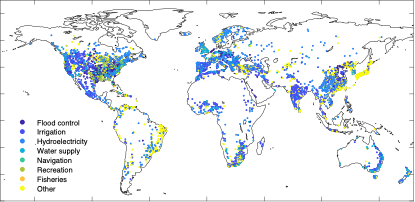
\includegraphics{Figures/基础数据/GranD-v1.1所包含水库的位置和主要用途.png}
\caption{GranD-v1.1所包含水库的位置和主要用途}
\label{fig:GranD-v1.1所包含水库的位置和主要用途}
\end{figure}
}


\subsubsection{全球水库水面面积数据}
全球水库水面面积数据来自Global Reservoir Surface Area Dataset(GRSAD),该数据集提供了全球6871个水库1984年至2015年的逐月水库面积变化数据(与GranD水库匹配)。该数据是基于Global Surface Water Dataset(GSWD)数据修正而得。\citet{pekel2016high} 使用1984$\sim$2015年300万张Landsat卫星图像创建了全球地表水数据集GSWD。但由于云、云阴影等因素的影响,利用Landsat对全球范围内单个水库进行长期水面变化分析会存在较大偏差。GRSAD修复了由于云层、云层阴影、地形阴影和扫描线校正器故障导致的像素污染,使每个时间序列中有效图像的数量平均提高了81\%~\citep{zhao2018automatic}。基于水库面积长期动态变化数据,可估算水库的防洪库容面积、正常库容面积和死库容面积。


\subsubsection{全球水库形状数据}

全球水库形状数据来源于Global Reservoir Geometry Database(ReGeom),该数据集包含了全球6824个水库的库容-面积-深度数据(与GranD水库匹配)。\citet{yigzaw2018new} 采用一种优化算法来确定每个水库的库容-面积-深度关系,该算法从五种可能的规则几何形状中迭代选择出最佳几何形状,以最小化水库总库容和表面积的估算误差。ReGeom数据集适用范围广泛,尤其适用于改进全球水文或地球系统模型中对水库动态的表达,特别是在水库信息有限或不精确的地区。数据集中包含了所有水库的近似几何数据(\texttt{ReGeomData\_WOW\_V1.xlsx})和每个水库的库容--面积--深度数据(\texttt{*.csv})。通过每个水库的防洪库容面积、正常库容面积和死库容面积,查找相应的库容--面积--深度数据,即可得到对应的防洪库容、正常库容和死库容。


\subsection{湖泊}
湖泊深度数据来自Lake-depth data set Version 2.0~\citep{kourzeneva2012global},数据为全球\ang{;;30} (约1公里)分辨率,经纬度网格,单时次数据。


\section{城市数据}\label{城市数据}

\subsection{城市地表覆盖}\label{城市地表覆盖}
城市地表覆盖数据采用MODIS-IGBP地表覆盖数据(章节 \ref{IGBP地表覆盖数据})中的城市覆盖类型作为判别依据。
模式利用该数据集区分不同年份网格城市覆盖类型,获得城市在网格中的覆盖度,反应不同年份的城市覆盖变化。


\subsection{城市类型划分}\label{城市类型划分}
模式对城市覆盖地区不同城市类型进行细分。城市类型分类数据目前采取两种方案:
\begin{enumerate}
    \item 传统的3类城市——高建筑街区 (Tall Building Distinct, TBD)、高密度(High Density, HD) 和中密度 (Medium Density, MD);
    \item 10类Local Climate Zone (LCZ 1-10)分类,如图~\ref{fig:LCZ分类图示}  所示。
\end{enumerate}

{
\begin{figure}[htbp]
\centering
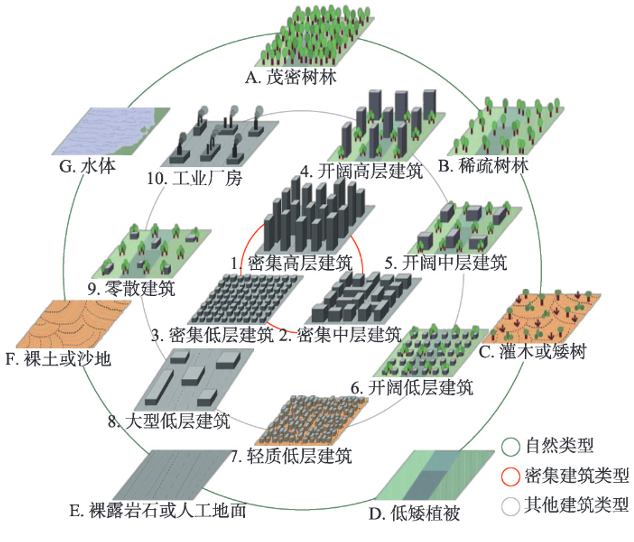
\includegraphics{Figures/基础数据/LCZ分类图示.png}
\caption{LCZ分类示意图}
\label{fig:LCZ分类图示}
\end{figure}
}


模式对于传统的城市类型分类与NCAR CLM--Urban Model~\citep{oleson2020parameterization} 相同,
根据 \citet{jackson2013parameterization} 的城市分类数据对全球城市化程度进行分类。该数据集中,城市化有三个水平,
及TBD、HD和MD,每1 km格点被划分为三个密度类别之一,通过该数据集对urban patch分为3类。其中,
TBD类城市指至少在1平方公里内,建筑高度全部大于或等于10层楼高且透水面比例较小(5$\sim$15\%);HD类城市建筑高度为3$\sim$10层,
透水面比例通常为5$\sim$25\%,这些地区通常为商业、住宅或工业区;MD类城市建筑高度通常为1$\sim$3层,且透水面比例较高,为20$\sim$60\%。
LCZ数据目前使用的 \citet{demuzere2022global} 全球LCZ分类数据,该数据空间分辨率为100米,
通过向轻量级随机森林模型输入大量标记训练区域和地球观测图像来生成,并对150个选定的功能城市地区采用自助交叉验证和专题基准测试评估了其质量。


\subsection{建筑形态及属性数据}\label{建筑形态及属性数据}
对于城市覆盖而言,建筑物的形态和物理性质(如反照率,导热率等)与其它地表覆盖类型完全不同,
这些物理性质取决于建筑物的材质及城市几何结构数据,比如: 不透水面比例分布(impervious fraction)、
建筑物屋顶面比例分布(roof fraction)、建筑物高度(building height)以及街区宽高比(H/W ratio)、反照率、发射率、导热率以及比热容等等。
目前使用 \citet{oleson2020parameterization} 基于 \citet{jackson2013parameterization} 的建筑数据开发的NCAR城市工具
(Toolbox for Human-Earth SystemIntegration \& Scaling (THESIS) toolset, \url{http://www.cgd.ucar.edu/iam/projects/thesis/thesis-urbanproperties-tool.html})
为模式生成各类城市形态以及物理性质输入参数。
该工具根据一定规则将全球所有国家分为33类 (图~\ref{fig:地区分类}),并根据传统城市分类进一步划分,不同类的国家不同类型建筑具有不同的性质。
%
而LCZ分类本身包含了一些建筑材料信息,不同地区的同类LCZ虽然有差别但是可能不会太大,
因此LCZ形态参数目前采用典型值设定,该部分数据一部分来源于~\citet{stewart2014evaluation},另一部分参考了WRF中的参数设置,LCZ参数如表 \ref{tab:lcz局地气候区建筑属性参数}所示。
{
\begin{figure}[htbp]
\centering
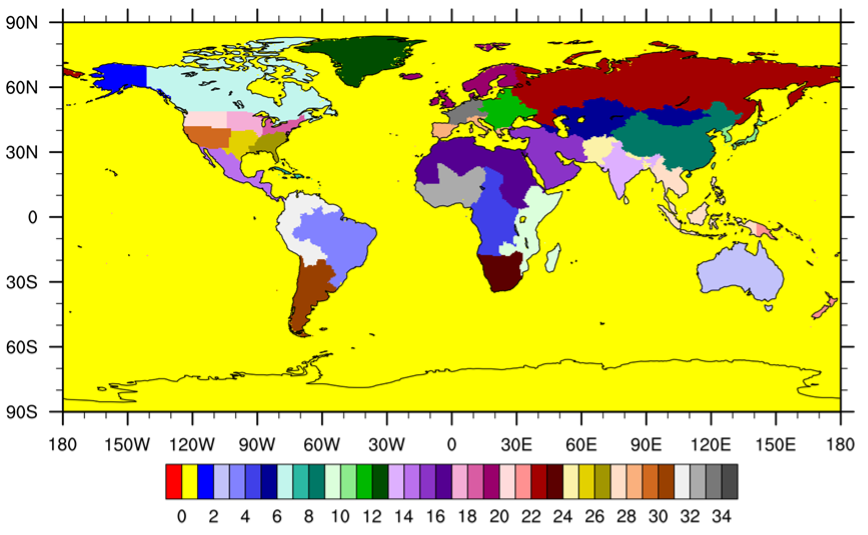
\includegraphics{Figures/基础数据/地区分类.png}
\caption{地区分类示意图}
\label{fig:地区分类}
\end{figure}
}


\subsection{建筑高度与建筑比例数据}\label{建筑高度与建筑比例数据}
建筑高度和建筑比例数据采用\citet{li2022global}等人发布的数据,该数据利用随机森林模型使用世界各地的参考数据进行训练得到。为了增加代表性,\citet{li2022global}对参考数据进行了人工分类和补充。该数据分辨率为1km,相比于其他陆面模型使用的根据区域或者LCZ类型查找表赋值建筑高度和比例的方法,该数据作为格点数据,精度较高,能更加真实的还原城市内部建筑的分布以及异质性。

\subsection{人口数据}\label{人口数据}
人口数据目前使用由美国能源部橡树岭国家实验室(ORNL)推出的LandScan数据,该数据采用地理信息系统与遥感影相结合的创新方法,在1km网格分辨率范围内,获取24小时内平均人口分布状况,LandScan是最好的全球人口动态统计分析数据集之一,该数据空间分辨率高(1km),时间可覆盖2000-2022年。

\subsection{城市树覆盖数据}\label{城市树覆盖数据}
NCAR CLM城市数据集比较全面的描述了全球城市的形态特征和物理性质,但是其城市数据缺少关于植被(树)和水体的描述,
LCZ分类虽然有植被描述但通常是一个范围值。由于城市只占全球陆地的1\%左右,相比于自然地表,在大尺度上城市占比仍然比较小,
因此在补充城市内部的植被覆盖数据时,需要尽量选择高分辨率的数据。否则,如果分辨率过低,城市中的植被等信息很可能无法识别。
GFCC Tree Cover (\url{https://lpdaac.usgs.gov/products/gfcc30tcv003/}) 提供了
2000年、2005年、2010年和2015年四个年代的全球树木覆盖度信息,分辨率为30 m,可用于了解森林变化。
该数据的投影方式为UTM,与陆面模式使用的等经纬度网格不同,需对数据进行投影转换,由UTM投影转换为经纬度投影 ($\sim$0.00025\textdegree)。
经过投影转换后,通过对全球数据每个区域的文件进行读取,并统计500 m 
 ($\sim$0.0041667\textdegree)分辨率下30 m高分辨网格植被总占比,
求平均得到500 m分辨率下城市格点的树覆盖数据作为城市模式的基础输入数据。


\subsection{城市内水体数据}\label{城市内水体数据}
基于与城市树覆盖同样的原因,水体数据也需要尽量选择高分辨率数据,30米全球地表覆盖数据GlobeLand30是中国研制的30 m空间分辨率全球地表覆盖数据,
2014年发布GlobeLand30 2000和2010版。自然资源部于2017年启动对该数据的更新。目前,GlobeLand30 2020版已发布 (\url{http://www.globallandcover.com/})。
除极地地区外,GlobeLand30同样采用了UTM投影,因此需要进行投影转换,
其中数据覆盖如图~\ref{fig:GlobeLand30数据覆盖示意图} 所示 (除2020年外,其他年份不包含极地地区数据)。
该数据集水体精度最高,达到了92.09\%~\citep{陈军2017},且时空分辨率高,
因此投影转换后用同样的方法生成了水体覆盖度数据作为城市模式的原始数据。

{
\begin{figure}[htbp]
\centering
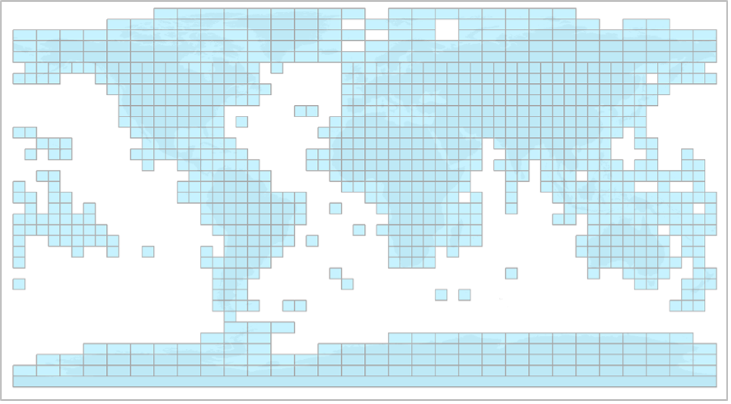
\includegraphics{Figures/基础数据/GlobeLand30数据覆盖示意图.png}
\caption{GlobeLand30数据覆盖示意图}
\label{fig:GlobeLand30数据覆盖示意图}
\end{figure}
}


\subsection{城市树高数据}\label{城市树高数据}
在CoLM2014版本中,树高数据采用\cite{simard2011mapping}发布的全球树高数据,该数据虽然应用广泛,但是分辨率较低(1km),无法满足城市模拟的需求,近年来,关于树高的高分辨率数据发展迅速,\cite{potapov2021mapping}利用GEDI卫星数据反演的树高数据具有较高的空间分辨率(30m,),但是由于卫星运行轨道限制,该数据目前只发布了$51.6°N$ $\sim$ $51.6°S$范围内的数据。\cite{lang2022global}则开发了一种从Sentinel-2光学图像中检索冠层高度的深度学习模型,该模型可以有效降低卫星观测树高偏低的问题,\cite{lang2022global}利用该模型并结合GEDI 30m树高数据生成了全球10m树高地图。相比于GEDI数据,该数据更全(全球),同时改善了GEDI偏低的问题,并且分别率更高(10m),因此将该数据集作为城市树高基础数据。


\subsection{城市LAI/SAI数据}\label{城市LAISAI数据}
城市模式中,植被另一个比较重要的参数——树木的LAI目前采取插值方法计算得到。主要因为目前LAI没有高于500m分辨率的数据,大部分遥感LAI数据为500m甚至1km(比如MODIS LAI),然而在城市中,由于城市中建筑物的遮掩,这种分辨率下卫星观测的城市LAI存在一定问题,但是作为描述植被的重要参数,LAI数据是不可或缺的。因此为了补充该数据,目前模式中城市LAI/SAI数据是根据格点内其它PFTs(只考虑树,即1-9类PFT)的LAI/SAI生成,具体方法为通过城市树高与PFTs树高比值插值并加权平均计算城市LAI/SAI,方法如下:
\begin{equation}
LAI_{urb}=\sum_{i=1}^{9} LAI_{PFT_{i}} \cdot \frac{HTOP_{urb}}{HTOP_{PFT_{i}}} \cdot PCT_{PFT_{i}}
\end{equation}
\begin{equation}
SAI_{urb}=\sum_{i=1}^{9} SAI_{PFT_{i}} \cdot \frac{HTOP_{urb}}{HTOP_{PFT_{i}}} \cdot PCT_{PFT_{i}}
\end{equation}
其中$LAI_{PFT_{i}}$($SAI_{PFT_{i}}$)为PFT的LAI(SAI),$HTOP_{urb}$和 $HTOP_{PFT_{i}}$分别为城市树高和PFT树高,$PCT_{PFT_{i}}$为PFT占比。$HTOP_{urb}$分辨率为500m,PFT占比、LAI/SAI以及PFT树高均为0.5°分辨率,通过插值计算后便得到500m分辨率下LAI/SAI数据。


\section{作物数据}

\subsection{作物种类分布数据}\label{作物种类分布数据}



\subsection{施肥数据}\label{施肥数据}



\subsection{播种时间数据}\label{播种时间数据}



\subsection{灌溉方式数据}\label{灌溉方式数据}
灌溉模拟所需的灌溉方式数据来源于~\citet{yao2022Irrigation}全球灌溉方式地图数据,数据中共包括了32种灌溉作物的灌溉方式分布,每种作物在数据网格中仅考虑一种灌溉方式(滴灌、喷灌、漫灌)。~\citet{jagermeyr2015irrigation}采用决策树算法对AQUASTAT数据\citep{fao2014aquastat}进行了重处理,该算法根据不同作物灌溉面积、土壤类型、作物特性、社会经济等要素,划分了全球14种CFT的灌溉方式(每种作物在网格上均可有3种不同的灌溉方式),分辨率为0.5\textdegree $\times$0.5\textdegree。\citep{yao2022Irrigation},则进一步将该数据中14种CFT与CLM5中的32种灌溉作物CFT进行匹配,并对数据进行重采样,得到新的全球灌溉方式数据。

\section{生物地球化学数据}

\subsection{氮沉降数据}\label{氮沉降数据}
氮沉降是陆地生态系统的重要氮输入之一。近几十年来,人类活动造成大气氮沉降增加对生态系统生物地球化学循环产生了重要影响。由于区域地表氮沉降数据尚无法利用卫星直接观测得到,目前生物地球化学循环模式更多地利用大气模式或地球系统模式模拟得出。CoLM生物地球化学循环模块的氮沉降输入是$\mathrm{NO_y}$和$\mathrm{NH_x}$的总和,数据来源于CESM-WACCM的CMIP6历史时期和未来SSP情景模拟的集合平均。氮沉降历史时期数据包含1849年到2013年的时空变化,氮沉降未来时期数据包含1849--2101年的时空变化,未来情景包括SSP126,SSP245,SSP370和SSP585四种情景的预测模拟结果。数据的空间分辨率为0.9375\textdegree\ $\times$ 1.25\textdegree,数据在月尺度上刻画大气氮沉降的季节和年际变化。


\subsection{土壤含氧量数据}\label{土壤含氧量数据}



\subsection{闪电频率数据}\label{闪电频率数据}



\subsection{国民生产总值数据}\label{国民生产总值数据}



\subsection{泥炭地比例数据}\label{泥炭地比例数据}



\subsection{火灾峰值月份数据}\label{火灾峰值月份数据}



\subsection{地表臭氧浓度数据}\label{地表臭氧浓度数据}



%\end{地表输入数据}
